%
\documentclass[11pt]{thesis} % draft

\title{Algorithmic Meta-Creativity}
\author{Fania Raczinski}
\date{March 2015}

% Test

\begin{document}

\subsubsection{Manipulation}

Within the manipluation category, (different representations of) sounds are pataphysicalised directly. There are several approaches to this, such as making changes to sound wave forms (an antinomy pataphysicalisation for example could be to invert a sound wave, i.e. where there was silence there is now noise and vice versa). These manipulations could be applied to specific sections only or the complete sound wave. This kind of manipluation could also be applied to musical scores. Changes might also happen in given compositions of music of multiple instruments (as opposed to pataphysicalising the composition process itself which is covered in section~\ref{s:composition}\marginpar{§~\ref{s:composition}}).

\begin{figure}[!htbp]
\centering
  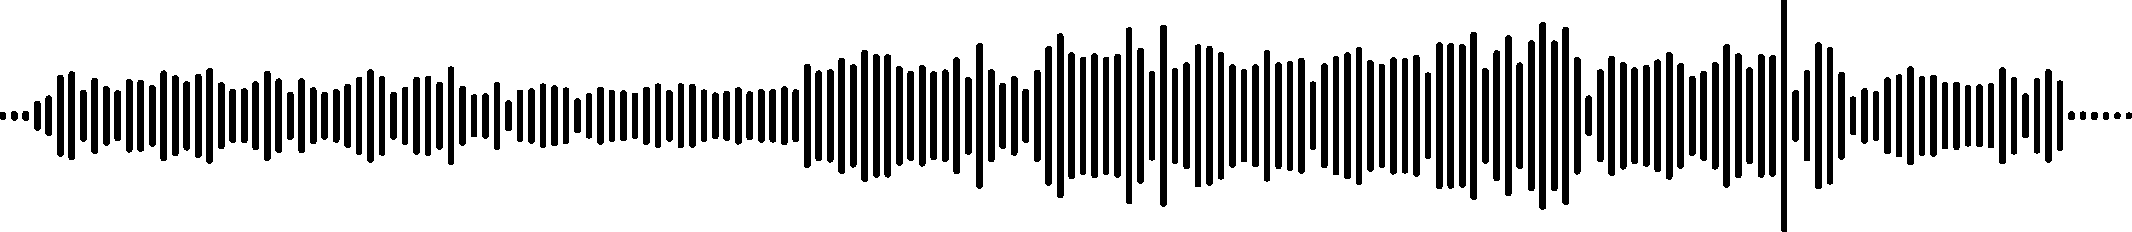
\includegraphics[width=\linewidth]{simplewave.pdf}
\caption[Sound wave of \textit{La Chanson Du D{\'e}cervelage}]{Sound wave of \textit{La Chanson Du D{\'e}cervelage} \autocite[][Track 1]{UbuWebPata}}
\end{figure}

``Cymbalum Pataphysicum Classiques Pataphysics 01 La Chanson Du Decervelage''
Tracks 1 and 5 were recorded on 6 January 1951 at the studio of Mr. Gruber, boulevard Pasteur in Reims.
in \autocite[][Track 1]{UbuWebPata}

Generated by 


- change pitch, compressing?, change of wave form/type (from sine wave to square wave), MIDI,  




The Web Audio API does ``include the capabilities found in modern game audio engines as well as some of the mixing, processing, and filtering tasks that are found in modern desktop audio production applications'' \autocite{Adenot2017}.

an example of using this API to synthesise sounds is described by Misuary \autocite{Misuary2016}



\autocite{soundcloud}

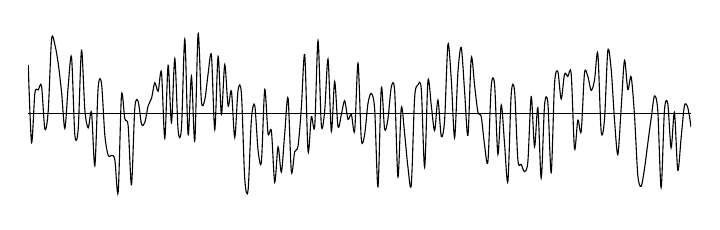
\begin{tikzpicture}[samples=200, domain=0:5*360]
  \begin{axis}[
    width=10cm, height=4cm,
    enlarge x limits=false,
    xtick=\empty,
    axis lines*=middle,
    hide y axis
  ]
  \addplot [no markers, smooth] {sin(x)+rand*2};
  \end{axis}
\end{tikzpicture}

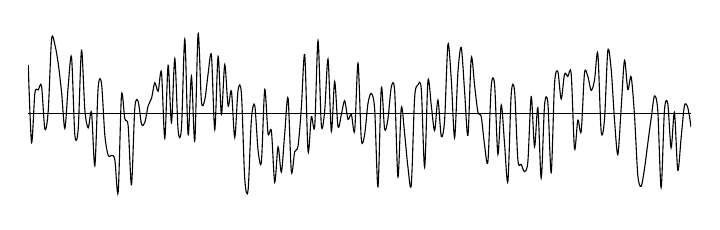
\begin{tikzpicture}[samples=200, domain=0:5*360]
  \begin{axis}[
    width=10cm, height=4cm,
    enlarge x limits=false,
    xtick=\empty,
    axis lines*=middle,
    hide y axis
  ]
  \addplot [no markers, smooth] {sin(x)+rand*2};
  \end{axis}
\end{tikzpicture}

\end{document}
